\subsection{Tuning of ESKF for real data}
The next step was to see how the error state Kalman filter would perform on actual real life data. The available dataset contains IMU and GNSS measurements of a unmanned aerial vehicle (UAV) remotely controlled by an operator. The flight path of the UAV as seen from the GNSS measurements is shown in figure \ref{fig:real-track}.
\begin{figure}[H]
\centering
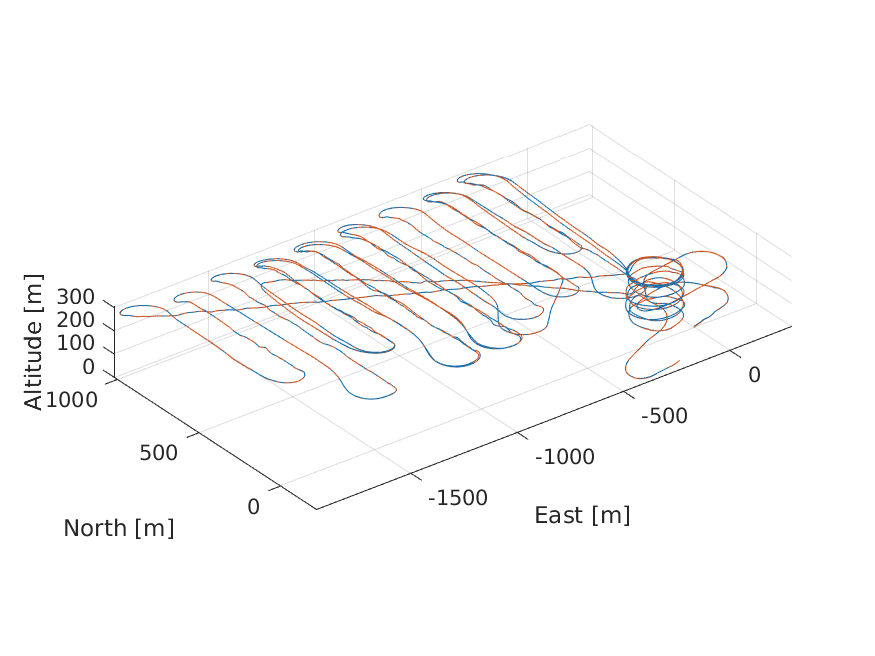
\includegraphics[width=0.6\textwidth]{plots/a2-real-track}
\caption{UAV Track}
\label{fig:real-track}
\end{figure}
